
\chapter{特殊张量}

除了秩或阶之外，有些张量还具有特殊结构，从而拥有一些很好的性质，例如可以快速缩并。
下面给出若干例子。


\section{快速 Kronecker 乘法}

假设我们想计算 $(A_1\otimes A_2\cdots A_n)x$，
其中 $A_i$ 是 $a_i \times a_i$ 矩阵，且 $x \in \R^{a_1 a_2 \cdots a_n}$。
如果先计算 Kronecker 积，再做矩阵-向量乘法，就需要 $(a_1\cdots a_n)^2$ 的时间。

相反，我们可以把 $x$ 重塑为一个 $a_1 \times \cdots a_n$ 张量，并执行乘法
\[
   \begin{tikzpicture}[baseline=-.25em]
      \node (A) at (1,.5) {$A_1$};
      \node (B) at (1,0) {$A_2$};
      \node (C) at (1,-0.4) {$\vdots$};
      \node (D) at (1,-1.1) {$A_n$};
      \node (x) at (2,0) {$X$};
      \draw (A) -- ++(-.6,0) node[midway, above, font=\tiny] {$a_1$};
      \draw (B) -- ++(-.6,0)node[midway, above, font=\tiny] {$a_2$};
      \draw ($(C.west)+(0,-.1)$) -- ++(-.4,0);
      \draw (D) -- ++(-.6,0) node[midway, below, font=\tiny] {$a_n$};
      \draw (A) -- (x) node[midway, above, font=\tiny] {$a_1$};
      \draw (B) -- (x);
      \draw ($(C.east)+(0,-.1)$) -- (x);
      \draw (D) -- (x) node[midway, below right, font=\tiny] {$a_n$};
   \end{tikzpicture}
%\quad\text{in time} lv
\]
也就是逐一缩并这些 $a_i$ 边。
这需要时间
\[
a_1^2(a_2\cdots a_n)
+ a_2^2(a_1a_3\cdots a_n)
+ \dots
+ a_n^2(a_1\cdots a_{n-1})
= (a_1 + \dots + a_n)(a_1 \cdots a_n),
\]
正如后面会看到的，这是许多快速算法的基础。

\section{Hadamard 变换}

Hadamard 矩阵定义为
$
H_{2^n}
= H_2^{\otimes n}
= H_2 \otimes \dots\otimes H_2
$
其中 $H_2=\smat{1 & 1 \\ 1 & -1}$。
例如
\[
  \renewcommand*{\arraystretch}{1}
  H_4 =
  H_2 \otimes H_2
= \begin{bmatrix}
   H_{2}
   & H_{2}
   \\ H_{2}
   & -H_{2}
\end{bmatrix}
=  \begin{bmatrix}
    1 &  1 &  1 &  1\\
    1 & -1 &  1 & -1\\
    1 &  1 & -1 & -1\\
    1 & -1 & -1 &  1
  \end{bmatrix}.
\]
它给出了如下非常简单的张量图表示：
\[
H_{2^n} = 
   \begin{tikzpicture}[baseline=-.25em]
      \node[triangle, rotate=180] (F0) at (0,0) {};
      \node (A) at (1,.5) {$H_2$};
      \node[triangle] (F1) at (2,0) {};
      \node (B) at (1,0.1) {$\vdots$};
      \node (C) at (1,-.5) {$H_2$};
      \draw[double] (F0) -- ++(-.4,0);
      \draw[double] (F1) -- ++(.4,0);
      \draw (F0) -- (A) -- (F1);
      \draw (F0) -- (B) -- (F1);
      \draw (F0) -- (C) -- (F1);
   \end{tikzpicture}
   \,.
\]
快速 Hadamard 变换（Fast Hadamard Transform, FHT）通常递归地描述为：
\[
   \renewcommand*{\arraystretch}{1.3}
H_{2^n} x
= \begin{bmatrix}
   H_{2^{n-1}} 
   & H_{2^{n-1}} 
   \\ H_{2^{n-1}} 
   & -H_{2^{n-1}} 
\end{bmatrix}
\begin{bmatrix}
    x^{(1)}
    \\
    x^{(2)}
\end{bmatrix}
,
\]
其中 $\smat{ x^{(1)} \\ x^{(2)} }$ 是 $x$ 的前半部分和后半部分。
由于矩阵乘法中存在冗余（它只依赖于 $H_{2^{n-1}}x^{(1)}$ 和 $H_{2^{n-1}} x^{(2)}$），该算法可以在 $O(N\log N)$ 时间内计算 $H_N x$。

另一种做法是直接使用上面描述的一般事实，其中所有 $a_i = 2$。
于是“快速 Kronecker 乘法”方法需要时间 $(a_1 a_2\cdots a_n)(a_1+a_2+\cdots a_n) = 2 n \log_2 n$。


\section{Fourier 变换}

% A more common matrix is the Discrete Fourier Matrix.
%\\
%\\
离散 Fourier 矩阵由 $(F_N)_{i,j}=\omega^{ij}$ 定义，
其中 $\omega = e^{-2\pi i/N}$：
%We can write it out as
\[
   \renewcommand*{\arraystretch}{1}
F_N =
   \begin{bmatrix}
      1&1&1&1&\cdots &1 \\
      1&\omega&\omega^2&\omega^3&\cdots&\omega^{N-1} \\
      1&\omega^2&\omega^4&\omega^6&\cdots&\omega^{2(N-1)}\\ 1&\omega^3&\omega^6&\omega^9&\cdots&\omega^{3(N-1)}\\
      \vdots&\vdots&\vdots&\vdots&\ddots&\vdots\\
      1&\omega^{N-1}&\omega^{2(N-1)}&\omega^{3(N-1)}&\cdots&\omega^{(N-1)(N-1)}
   \end{bmatrix}
.
\]
使用前面介绍过的函数语法，并假设 $n$ 是向量 $[1, 2, \dots, N]$，另一种写法是：
\[
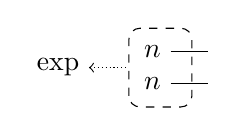
\begin{tikzpicture}
    % Place the exp text
    \node (exp) at (-.2,0) {$\exp$};
    
    \begin{scope}[xshift=1cm]
        % Draw the dashed rectangle
        \draw[dashed, rounded corners] (-.3,-0.5) rectangle (.5,0.5);
        % Add the n labels
        \node(n1) at (0,0.2) {$n$};
        \node(n2) at (0,-0.2) {$n$};
        \draw (n1) -- ++(.7,0);
        \draw (n2) -- ++(.7,0);
    \end{scope}
    
    % Draw the dotted arrow
    \draw[densely dotted, <-] (exp.east) -- ++(0.5,0);
\end{tikzpicture}
\]

Good-Thomas 快速 Fourier 变换（Fast Fourier Transform, FFT）使用基于中国剩余定理的分解：
\[
F_{N} = 
   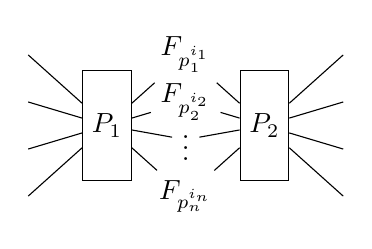
\begin{tikzpicture}[baseline=-1em, y=1.7em]
      \node[rectangle, draw, minimum height=4em] (P1) at (0,-.5) {$P_1$};
      \node (A) at (1,1) {$F_{p_1^{i_1}}$};
      \node[rectangle, draw, minimum height=4em] (P2) at (2,-.5) {$P_2$};
      \node (B) at (1,0) {$F_{p_2^{i_2}}$};
      \node (C) at (1,-.8) {$\vdots$};
      \node (D) at (1,-2) {$F_{p_n^{i_n}}$};
      \draw (-1,1) -- (P1) -- (A) -- (P2) -- (3, 1);
      \draw (-1,0) -- (P1) -- (B) -- (P2) -- (3, 0);
      \draw (-1,-1) -- (P1) -- (C) -- (P2) -- (3, -1);
      \draw (-1,-2) -- (P1) -- (D) -- (P2) -- (3, -2);
   \end{tikzpicture}
   \,,
\]
其中 $N = p_1^{i_1} p_2^{i_2} \cdots p_n^{i_n}$ 是 $N$ 的素因数分解，$P_1$ 和 $P_2$ 是某些置换矩阵。

使用快速 Kronecker 乘法，该算法需要 $(p_1^{i_1}+\dots+p_n^{i_n}) N$ 时间。
通过给 $x$ 补零，可以把 $N$ 增大一个常数倍，从而得到一串 $n=O(\log(N)/\log\log(N))$ 个素数，其和为 $\sim n^2/\log n = O(\log(N)^2)$。
因此完整算法需要 $O(N \log(N)^2)$ 时间。
接下来我们会看到如何把它降低到 $O(N\log N)$。

经典的 Cooley-Tukey FFT 算法使用如下递归：
\[
   \renewcommand*{\arraystretch}{1.3}
F_N =
\begin{bmatrix}
I & I \\
I & -I
\end{bmatrix}
\begin{bmatrix}
I & 0 \\
0 & D_{N/2}
\end{bmatrix}
\begin{bmatrix}
F_{N/2} & 0 \\
0 & F_{N/2}
\end{bmatrix}
\begin{bmatrix}
\text{even-odd} \\
\text{permutation}
\end{bmatrix}
,
\]
其中 $D_N = [1, w^N, w^{2N}, \dots]$。
偶奇置换会把所有偶数位置的值移到开头。
如果把 $I_{2^n}$ 重塑为 $I_2\otimes\dots\otimes I_2$，这个置换就是
$
P_N = 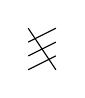
\begin{tikzpicture}[baseline=.5em, x=1em, y=.5em]
    \draw (0,0) -- (1, 1);
    \draw (0,1) -- (1, 2);
    \draw (0,2) -- (1, 3);
    \draw (0,3) -- (1, 0);
\end{tikzpicture}
$,
或者用 pytorch 写作：\texttt{x.permute([3,0,1,2])}。
还要注意，
$\smat{I&I\\I&-I} = H_2 \otimes I$ 且 $\smat{F_{N/2} & 0\\0&F_{N/2}}=I_2 \otimes F_{N/2}$。
因此可以用张量图记号写成：
\begin{align*}
F_N =
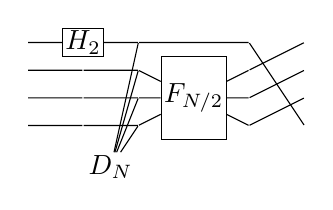
\begin{tikzpicture}[baseline=-2em, x=2em, y=1em, inner sep=1pt]
    \node[rectangle,draw] (H) at (0,0) {$H_2$};
    \node[inner sep=0pt, minimum size=0pt] (l1) at (0,-1) {};
    \node[inner sep=0pt, minimum size=0pt] (l2) at (0,-2) {};
    \node[inner sep=0pt, minimum size=0pt] (l3) at (0,-3) {};
    \node[inner sep=0pt, minimum size=0pt] (L0) at (-1,0) {};
    \node[inner sep=0pt, minimum size=0pt] (L1) at (-1,-1) {};
    \node[inner sep=0pt, minimum size=0pt] (L2) at (-1,-2) {};
    \node[inner sep=0pt, minimum size=0pt] (L3) at (-1,-3) {};
    \node[inner sep=0pt, minimum size=0pt] (b0) at (1,0) {$\sbullet$};
    \node[inner sep=0pt, minimum size=0pt] (b1) at (1,-1) {$\sbullet$};
    \node[inner sep=0pt, minimum size=0pt] (b2) at (1,-2) {$\sbullet$};
    \node[inner sep=0pt, minimum size=0pt] (b3) at (1,-3) {$\sbullet$};
    \node (D) at (.5,-4.5) {$D_N$};
    \node[rectangle,draw,minimum height=3em] (F) at (2,-2) {$F_{N/2}$};
    \node[inner sep=0pt, minimum size=0pt] (r0) at (4,0) {};
    \node[inner sep=0pt, minimum size=0pt] (r1) at (4,-1) {};
    \node[inner sep=0pt, minimum size=0pt] (r2) at (4,-2) {};
    \node[inner sep=0pt, minimum size=0pt] (r3) at (4,-3) {};
    \node[inner sep=0pt, minimum size=0pt] (s0) at (3,0) {};
    \node[inner sep=0pt, minimum size=0pt] (s1) at (3,-1) {};
    \node[inner sep=0pt, minimum size=0pt] (s2) at (3,-2) {};
    \node[inner sep=0pt, minimum size=0pt] (s3) at (3,-3) {};
    \draw (b0) -- (D);
    \draw (b1) -- (D);
    \draw (b2) -- (D);
    \draw (b3) -- (D);
    \draw (L0) -- (H) -- (b0) -- (s0) -- (r3);
    \draw (L1) -- (l1) -- (b1) -- (F) -- (s1) -- (r0);
    \draw (L2) -- (l2) -- (b2) -- (F) -- (s2) -- (r1);
    \draw (L3) -- (l3) -- (b3) -- (F) -- (s3) -- (r2);
\end{tikzpicture}
&=
\begin{tikzpicture}[baseline=-2em, x=2em, y=1em, inner sep=1pt]
    % Draw H nodes and connections
    \foreach \i in {0,...,3} {
        \node[rectangle,draw] (H\i) at (2*\i,-\i) {$H_2$};
        \node[inner sep=0pt, minimum size=0pt] (l\i) at (0,-\i) {};
        \node[inner sep=0pt, minimum size=0pt] (L\i) at (-1,-\i) {};
        \node[inner sep=0pt, minimum size=0pt] (s\i) at (7,-\i) {};
        \node[inner sep=0pt, minimum size=0pt] (r\i) at (8,-\i) {};
    }
    % Draw D nodes and connections to sbullets
    \foreach \i in {0, 1, 2} {
        \node (D\i) at (0.5+\i*2,-4.5) {$D_{N/2^\i}$};
        \foreach \k in {\i,...,3} {
            \node[inner sep=0pt, minimum size=0pt] (b\i\k) at (1+\i*2,-\k) {$\sbullet$};
            \draw (b\i\k) -- (D\i);
        }
    }
    \draw (L0) -- (H0) -- (b0) -- (s0) -- (r3);
    \draw (L1) -- (l1) -- (b1) -- (H1) -- (b11) -- (s1) -- (r2);
    \draw (L2) -- (l2) -- (b2) -- (b12) -- (H2) -- (b22) -- (s2) -- (r1);
    \draw (L3) -- (l3) -- (b3) -- (b13) -- (b23) -- (H3) -- (s3) -- (r0);
\end{tikzpicture}
%\\&=
%\begin{tikzpicture}[baseline=-2em, x=2em, y=1em, inner sep=1pt]
%    % Draw H nodes and connections
%    \foreach \i in {0,...,3} {
%        \node[rectangle,draw] (H\i) at (2*\i,-3+\i) {$H_2$};
%        \node[inner sep=0pt, minimum size=0pt] (l\i) at (0,-\i) {};
%        \node[inner sep=0pt, minimum size=0pt] (L\i) at (-1,-\i) {};
%        \node[inner sep=0pt, minimum size=0pt] (s\i) at (7,-\i) {};
%        \node[inner sep=0pt, minimum size=0pt] (r\i) at (-2,-\i) {};
%    }
%    % Draw D nodes and connections to sbullets
%    \foreach \i in {0, 1, 2} {
%        \node (D\i) at (0.5+\i*2,-4.5) {$D_{N/2^\i}$};
%        \foreach \k in {\i,...,3} {
%            \node[inner sep=0pt, minimum size=0pt] (b\i\k) at (1+\i*2,-\k) {$\sbullet$};
%            \draw (b\i\k) -- (D\i);
%        }
%    }
%    \draw (r3) -- (L0) -- (H3) -- (b0) -- (s0);
%    \draw (r2) -- (L1) -- (l1) -- (b1) -- (H2) -- (b11) -- (s1);
%    \draw (r1) -- (L2) -- (l2) -- (b2) -- (H1) -- (b12) -- (b22) -- (s2);
%    \draw (r0) -- (L3) -- (H0) -- (l3) -- (b3) -- (b13) -- (b23) -- (s3);
%\end{tikzpicture}
.
\end{align*}
由于可以在线性时间内完成置换矩阵和对角矩阵的乘法，所以 $O(n\log n)$ 的时间复杂度可以由 Hadamard 情形中的同一论证推出。

注意这里有许多对称性；例如，由于该矩阵是对称的，可以通过转置（水平翻转）得到对称形式。
也可以把置换推到左侧。

我们不必把矩阵二等分，也可以把它三等分、四等分，等等。
使用这种广义 Cooley-Tukey 算法，可以得到下图：
\[
   F_N =
\begin{tikzpicture}[baseline=-2em, x=2em, y=1em, inner sep=1pt]
    % Draw H nodes and connections
    \foreach \i in {0,...,3} {
        \node[rectangle,draw] (H\i) at (2*\i,-\i) {$F_{n_\i}$};
        \node[inner sep=0pt, minimum size=0pt] (L\i) at (-1,-\i) {};
        \node[inner sep=0pt, minimum size=0pt] (s\i) at (7,-\i) {};
        \node[inner sep=0pt, minimum size=0pt] (r\i) at (8,-\i) {};
    }
    % Draw D nodes and connections to sbullets
    \node (D0) at (0.5+0*2,-4.5) {$\scriptstyle F^{(n_0, n_1n_2n_3)}$};
    \node (D1) at (0.5+2.2,-4.5) {$\scriptstyle F^{(n_1, n_2n_3)}$};
    \node (D2) at (0.5+2*2,-4.5) {$\scriptstyle F^{(n_2, n_3)}$};
    \foreach \i in {0, 1, 2} {
        \foreach \k in {\i,...,3} {
            \node[inner sep=0pt, minimum size=0pt] (b\i\k) at (1+\i*2,-\k) {$\sbullet$};
            \draw (b\i\k) -- (D\i);
        }
    }
    \draw (L0) -- (H0) -- (b0) -- (s0) -- (r3);
    \draw (L1) -- (b1) -- (H1) -- (b11) -- (s1) -- (r2);
    \draw (L2) -- (b2) -- (b12) -- (H2) -- (b22) -- (s2) -- (r1);
    \draw (L3) -- (b3) -- (b13) -- (b23) -- (H3) -- (s3) -- (r0);
\end{tikzpicture}
,
\]
其中 $n_0n_1n_2n_3 = N$。
这里我们把 $D_N$ 矩阵替换成了“广义”Fourier 矩阵 $F^{(a,b)}$；它定义为 $F^{(a,b)}_{j,k} = e^{-2\pi i j k/(ab)}$，并按需要进行了重塑。
在只分成两个大致满足 $n_1=n_2=\sqrt{N}$ 的部分这一简单情形中，它也称为“四步 FFT”（Four step FFT）或 Bailey 的 FFT 算法。

可以利用性质 $F_{a,bc} = F_{a,b} \bullet F_{a,c}^{1/b}$ 进一步化简该图：
\[
   F_N =
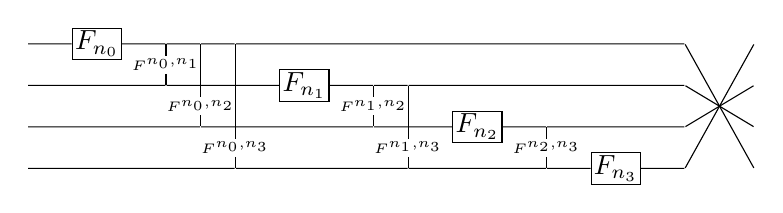
\begin{tikzpicture}[baseline=-2em, x=2.5em, y=1.5em, inner sep=1pt]
    % Draw H nodes and connections
    \foreach \i in {0,...,3} {
        \node[rectangle,draw] (H\i) at (3.25*\i-\i*\i/4,-\i) {$F_{n_\i}$};
        \node[inner sep=0pt, minimum size=0pt] (L\i) at (-1,-\i) {};
        \node[inner sep=0pt, minimum size=0pt] (s\i) at (8.5,-\i) {};
        \node[inner sep=0pt, minimum size=0pt] (r\i) at (9.5,-\i) {};
    }
    % Draw D nodes and connections to sbullets
    \foreach \i in {0, 1, 2} {
        \pgfmathtruncatemacro{\j}{\i+1}
        \foreach \k in {\j,...,3} {
            \node[inner sep=0pt, minimum size=0pt] (b\i\k) at (1/2+2.75*\i-\i*\i/4+\k/2,-\i) {$\sbullet$};
            \node[inner sep=0pt, minimum size=0pt] (c\i\k) at (1/2+2.75*\i-\i*\i/4+\k/2,-\k) {$\sbullet$};
        }
    }
    \node (D00) at (1,-.5) {$\scriptscriptstyle F^{n_0, n_1}$};
    \node (D01) at (1.5,-1.5) {$\scriptscriptstyle F^{n_0, n_2}$};
    \node (D02) at (2,-2.5) {$\scriptscriptstyle F^{n_0, n_3}$};
    \draw (b01) -- (D00) -- (c01);
    \draw (b02) -- (D01) -- (c02);
    \draw (b03) -- (D02) -- (c03);
    \node (D10) at (4,-1.5) {$\scriptscriptstyle F^{n_1, n_2}$};
    \node (D11) at (4.5,-2.5) {$\scriptscriptstyle F^{n_1, n_3}$};
    \draw (b12) -- (D10) -- (c12);
    \draw (b13) -- (D11) -- (c13);
    \node (D20) at (6.5,-2.5) {$\scriptscriptstyle F^{n_2, n_3}$};
    \draw (b23) -- (D20) -- (c23);
    % Horizontal connections
    \draw (L0) -- (H0) -- (b01) -- (b02) -- (b03) -- (s0) -- (r3);
    \draw (L1) -- (c01) -- (H1) -- (b12) -- (b13) -- (s1) -- (r2);
    \draw (L2) -- (c02) -- (c12) -- (H2) -- (b23) -- (s2) -- (r1);
    \draw (L3) -- (c03) -- (c13) -- (c23) -- (H3) -- (s3) -- (r0);
\end{tikzpicture}
.
\]
% This algorithm is actually slower (n (log n)^2), because the pair-wise D matrices are not actually faster.
在每次都分成 $2$ 份的简单情形中，这也称为“量子 FFT”（Quantum FFT）算法。

上面隐藏了一些细节，也就是说这些矩阵应当除以不同的 $N$。


注意，这个图可能与你见过的一些 FFT 图不同。
那些图通常长这样：
\[
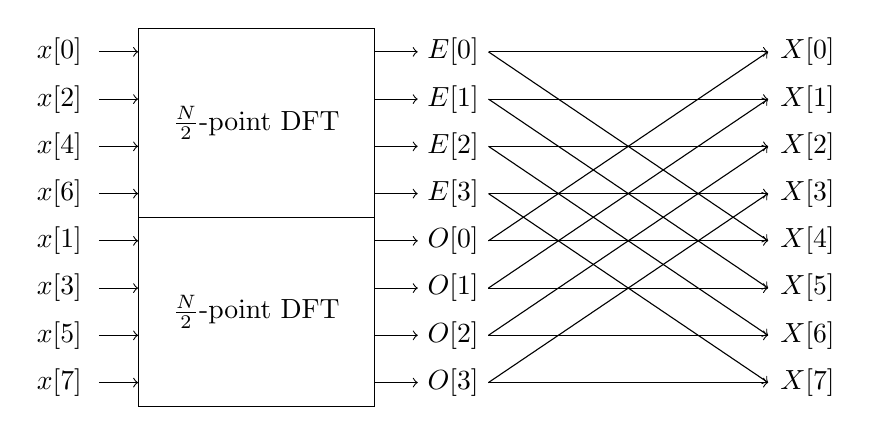
\begin{tikzpicture}
  % Draw N/2-point DFT blocks
  \draw (0, -2.1) rectangle (3, .3) node[midway] {$\frac{N}{2}$-point DFT};
  \draw (0, -4.5) rectangle (3, -2.1) node[midway] {$\frac{N}{2}$-point DFT};

  % Input nodes, even part
  \foreach \i in {0,2,4,6} {
    \node at (-1, - \i*0.3) {$x[\i]$};
    \draw[->] (-0.5, - \i*0.3) -- (0, - \i*0.3);
  }
  % Odd part
  \foreach \i in {1,3,5,7} {
    \node at (-1, - \i*0.3 - 2.1) {$x[\i]$};
    \draw[->] (-0.5, - \i*0.3 - 2.1) -- (0, - \i*0.3 - 2.1);
  }
  % Intermediate outputs E and O their edges
  \foreach \i in {0,1,2,3} {
    \node (E) at (4, - \i*0.6) {$E[\i]$};
    \draw[->] (3, - \i*0.6) -- (E.west);
    \draw[->] (E.east) -- (8, - \i*0.6);
    \draw[->] (E.east) -- (8, - \i*0.6 - 2.4);
  }
  \foreach \i in {0,1,2,3} {
    \node (O) at (4, - \i*0.6 - 2.4) {$O[\i]$};
    \draw[->] (3, - \i*0.6 - 2.4) -- (O.west);
    \draw[->] (O.east) -- (8, - \i*0.6);
    \draw[->] (O.east) -- (8, - \i*0.6 - 2.4);
  }
  % Output nodes X
  \foreach \i in {0,...,7} {
    \node at (8.5, - \i*0.6) {$X[\i]$};
  }
\end{tikzpicture}
\]
并且有 $2^n$ 行。
而张量图只有 $n$ 行（也就是 $\log_2 N$ 行）。

\subsubsection{多维 Fourier 变换}
这只是沿每个轴分别做 Fourier 变换。

\subsection{Vandermonde 矩阵}
可以定义“Vandermonde 函数”（Vandermonde Function）$\mathrm{vm}_N(x) = (1, x, x^2, \dots, x^{N-1})$。
于是 Vandermonde 矩阵 $V_{i,j}=x_i^j$ 定义为：
\[
   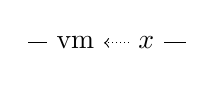
\begin{tikzpicture}
      \node(vm) at (0,0) {vm};
      \node(x) at (.9,0) {$x$};
      \draw[densely dotted, ->] (x) -> (vm);
      \draw (x) -- ++(.5,0);
      \draw (vm) -- ++(-.6,0);
   \end{tikzpicture}
\]
如果 $a\in\R^N$ 是多项式 $P(x)=a_0 + a_1 x + \dots$ 的系数向量，那么可以如下得到“批量求值”（batch evaluation）向量 $(P(x_1), P(x_2), \dots)$：
\[
   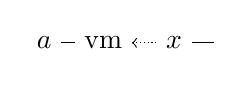
\begin{tikzpicture}
      \node(a) at (-.75,0) {$a$};
      \node(vm) at (0,0) {vm};
      \node(x) at (.9,0) {$x$};
      \draw[densely dotted, ->] (x) -> (vm);
      \draw (x) -- ++(.5,0);
      \draw (vm) -- (a);
   \end{tikzpicture}
\]

使用上面描述的 FFT，可以快速完成这一过程（时间为 $O(n(\log n)^2)$）。
% <ref>{{cite book |last1=Von Zur Gathen |first1=Joachim |title=Modern computer algebra |last2=Jürgen |first2=Gerhard |publisher=[[Cambridge University Press]] |year=2013 |isbn=9781139856065 |at=Chapter 10 |author-link=Joachim von zur Gathen}}</ref>
思路是定义两个多项式，它们分别在前半部分点和后半部分点上为零：
\begin{align*}
   m_0(x)&=(x-x_1)\cdots(x-x_{n/2}) \quad\text{且}\\
   m_1(x)&=(x-x_{n/2+1})\cdots(x-x_{n}).
\end{align*}
然后使用多项式余数定理计算 $R_0 = P \bmod m_0$ 和 $R_1 = P \bmod m_1$；借助 FFT，这可以在 $O(n\log n)$ 时间内完成。
这意味着
\begin{align*}
   P(x) &= Q_0(x)m_0(x) + R_0(x) \quad\text{且}\\
   P(x) &= Q_1(x)m_1(x) + R_1(x)
\end{align*}
按构造成立，其中 $R_0$ 和 $R_1$ 是次数至多为 $n/2$ 的多项式。
由于 $m_0$ 和 $m_1$ 的定义方式，有
\begin{align*}
R_0(x_i) &= P(x_i) \quad\text{对 } i \le n/2 \quad\text{且}\\
R_1(x_i) &= P(x_i) \quad\text{对 } i > n/2.
\end{align*}
因此，要在所有 $n$ 个 $x_i$ 上计算 $P$，只需分别在两半点上计算较小的多项式 $R_0$ 和 $R_1$。
（多项式 $Q_0$ 和 $Q_1$ 可以忽略。）
这给出了一个满足 $T(n) = 2T(n/2) + n\log n$ 的分治算法，从而推出 $T(n)=O(n(\log n)^2)$。



\subsection{块矩阵}
Schur 补这类对象很有意思。
但我们能否用张量图说出一些有用的内容？

来自 The Matrix Cookbook：
考虑矩阵

\[
   \left[ \begin{array}{c|c} A_{11} & A_{12} \\ \hline A_{21} & A_{22} \end{array} \right]
\]

上面矩阵中块 $A_{11}$ 的 Schur 补是如下矩阵（在上面的文字中记为 $C_2$）

\[
   A_{22} - A_{21}A_{11}^{-1}A_{12}
\]

上面矩阵中块 $A_{22}$ 的 Schur 补是如下矩阵（在上面的文字中记为 $C_1$）

\[
   A_{11} - A_{12}A_{22}^{-1}A_{21}
\]

利用 Schur 补，可以把块矩阵的逆改写为

\[
   \left[ \begin{array}{c|c} A_{11} & A_{12} \\ \hline A_{21} & A_{22} \end{array} \right]^{-1}
= \left[ \begin{array}{c|c} I & 0 \\ \hline -A_{22}^{-1}A_{21} & I \end{array} \right] \left[ \begin{array}{c|c} (A_{11} - A_{12}A_{22}^{-1}A_{21})^{-1} & 0 \\ \hline 0 & A_{22}^{-1} \end{array} \right] \left[ \begin{array}{c|c} I & -A_{12}A_{22}^{-1} \\ \hline 0 & I \end{array} \right]
\]

在求解如下形式的线性方程组时，Schur 补很有用：

\[
   \left[ \begin{array}{c|c} A_{11} & A_{12} \\ \hline A_{21} & A_{22} \end{array} \right] \left[ \begin{array}{c} x_1 \\ x_2 \end{array} \right] = \left[ \begin{array}{c} b_1 \\ b_2 \end{array} \right]
\]

它给出关于 $x_1$ 的如下方程：

\[
   (A_{11} - A_{12}A_{22}^{-1}A_{21})x_1 = b_1 - A_{12}A_{22}^{-1}b_2
\]

当相应的逆存在时，可以先解出 $x_1$，再把它代入关于 $x_2$ 的方程以解出 $x_2$。

%\subsection{Hermitian Matrices and skew-Hermitian}
%Complex. Skip
%\subsection{Idempotent Matrices}
%Skip
%\subsection{Orthogonal matrices}
%Skip
%\subsection{Positive Definite and Semi-definite Matrices}
%Skip
%\subsection{Singleentry Matrix, The}
%Describes the matrix $J$.
%All of this is trivial with diagrams.
\subsection{对称、斜对称/反对称}
\label{sec:symmetric}

可以在这里介绍 Penrose 的对称张量？
% The best sources is probably
% https://www.mscs.dal.ca/%7Eselinger/papers/graphical-bib/public/Penrose-applications-of-negative-dimensional-tensors.pdf

\subsection{Toeplitz 矩阵}
可以在这里讨论卷积张量……
\subsection{单位矩阵、置换与移位}
不是特别有意思……
